\chapter{Background and Related Work} % (fold)
\label{chap:Background and Work}


\section{Multicast Protocols} % (fold)
\label{sec:Mutlicast Protocols}
Multicast communication refers to the simultaneous delivery of data towards an
    arbitrary number of destinations
    \cite{mc_routing_multimedia, mc_comm_multicomputer}.
Numerous network protocols have been developed to facilitate multicast
communication, encompassing both Network Layer as well as Application Layer
    implementations \cite{universal_mc, overlay_mc_routing}.
This chapter first distinguishes Multicast from other communication schemes.
Subsequently, various multicast protocols are introduced.

According to the OSI model \cite{osi1980} Layer 3, known as the Network Layer,
    is responsible for end-to-end delivery of data between nodes.
In computer networks data is transferred through \glspl{pdu}, composed of
    protocol specific control information (e.g. source and destination
    address), along with a payload carrying the actual data.
To establish a path from the sender to the destination(s), packets (Layer 3
    \glspl{pdu}) may traverse multiple intermediate nodes \cite{rfc791_ip}.
This process is called routing and can be classified into various schemes.
For the purpose of this thesis, our primary focus lies on the schemes depicted
    in \autoref{fig:multicast}.
\textit{Unicast} denotes a one-to-one association between a sender and a single
    destination.
\textit{Broadcast} disseminates packets to all nodes within the sender's
    broadcast domain (Layer 2) \cite{broadcast}.
Typically, IP Routers (Layer 3) serve as the boundary of a broadcast domain.
\textit{Multicast} transmits packets to a group of destinations, accommodating
    both one-to-many and many-to-many communication \cite{rfc1112_ip4mc}.
In contrast to Broadcast, Multicast does not necessarily deliver packets to all
    available nodes.
Furthermore, Multicast packets can be delivered beyond the sender's broadcast 
    domain, implying subsequent replication of the packets.

% This layer is responsible for end-to-end delivery of data between nodes across
%     interconnected networks.
% A network comprises interconnected nodes, each assigned a unique address within
%     this network \cite{rfc791_ip}. 
% Data delivery is achieved through the transmission of network packets,
%     consisting of a header containing the source and destination address, along
%     with a payload carrying the actual data.
% If the data size exceeds the maximum transfer unit of Layer 2, it is fragmented
%     into multiple packets and subsequently reassembled.

\begin{figure}[h]
    \begin{center}
        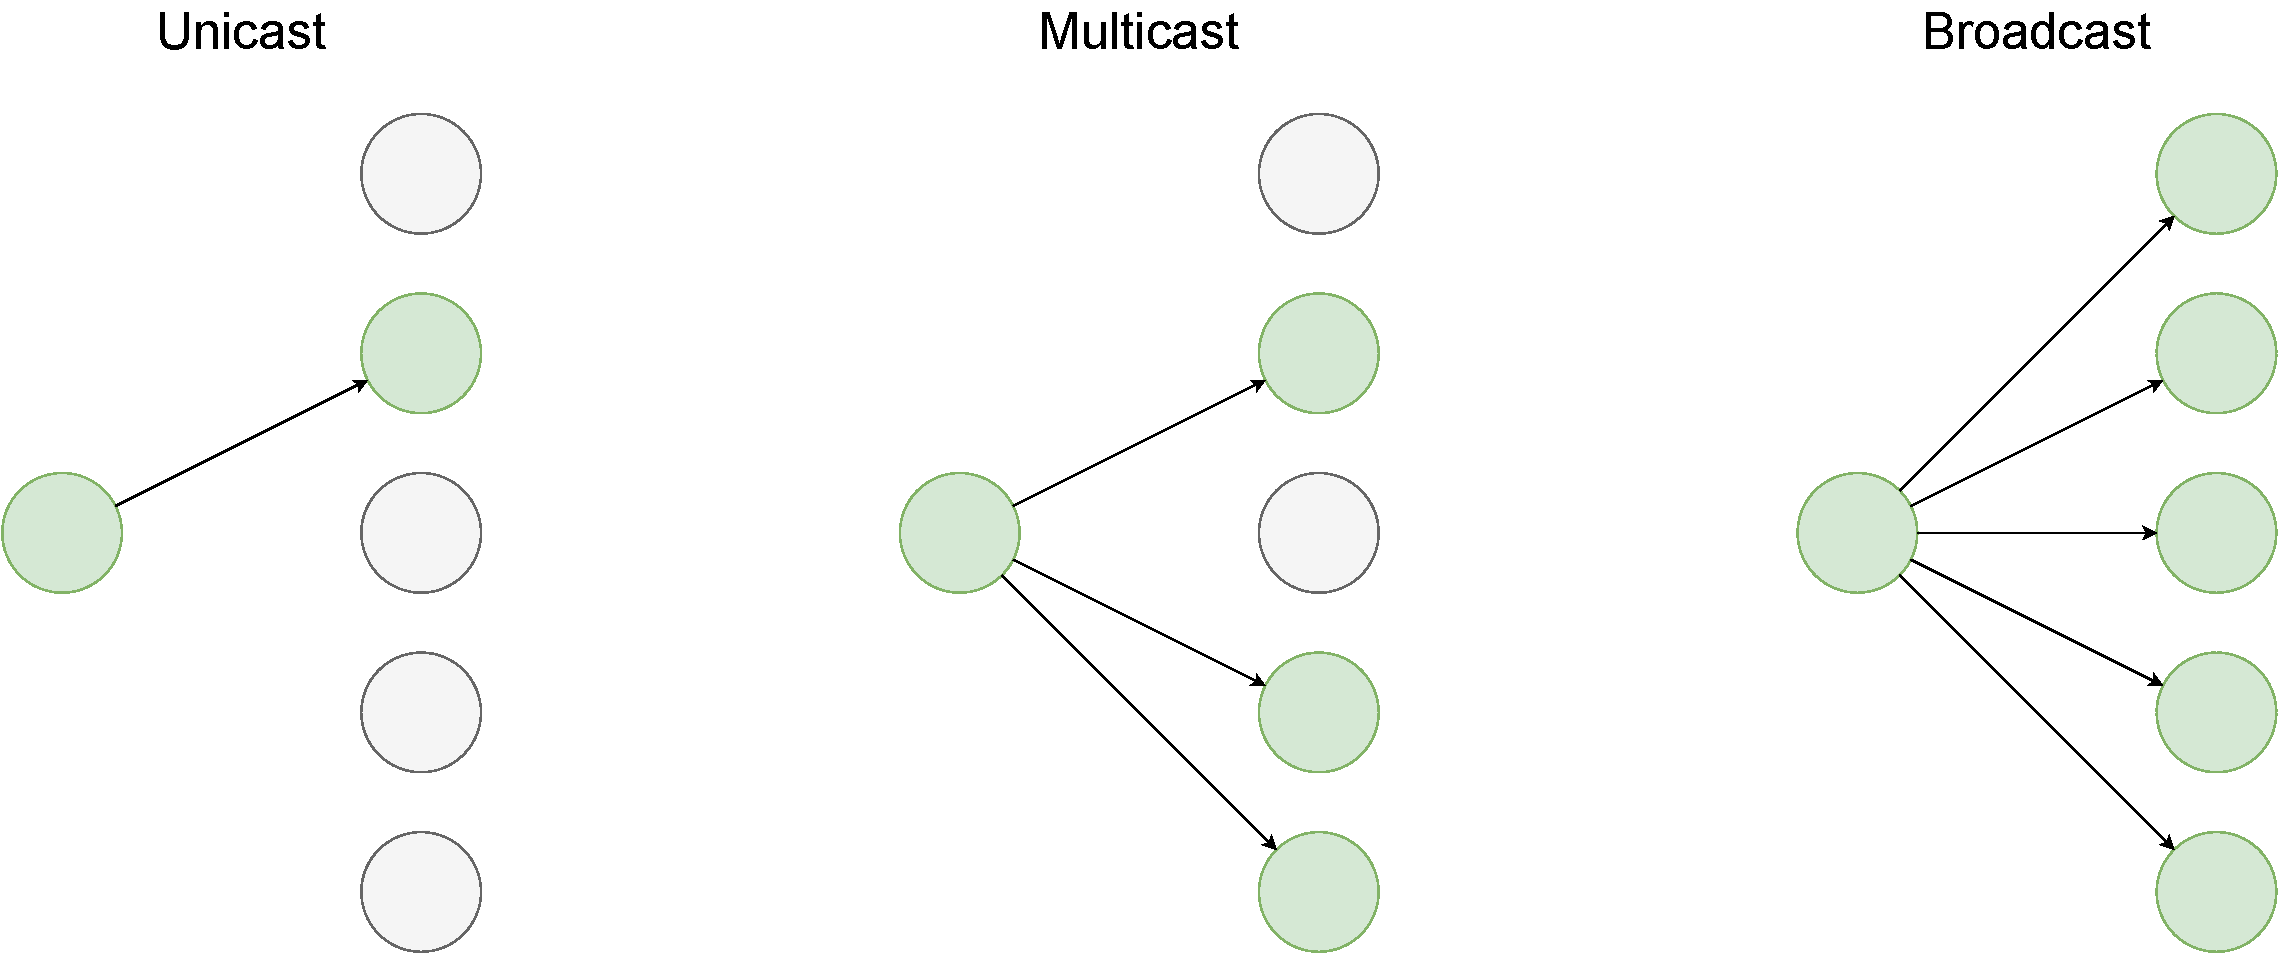
\includegraphics[width=0.85\textwidth]{multicast.pdf}
    \end{center}
    \caption{Network Layer: Routing schemes}
    \label{fig:multicast}
\end{figure}


\subsection{IP Multicast} % (fold)
\label{sub:IP Multicast}
Already in the late 1980s, \citeauthor{deering1990multicast}
    \cite{deering1990multicast} proposed an extension to the IP protocol, to
    facilitate efficient multipoint communication (\textit{1:n}, \textit{m:n}).
This extension is known as IP-Multicast and was first standardized in RFC 988
    (\citeyear{rfc988_initmc}) \cite{rfc988_initmc}.
IP-Multicast offers the advantage, to greatly reduce the bandwidth by condensing
    identical traffic into a single stream targeted to a so called ``Host
    Group'' \cite{rfc1112_ip4mc}.
IP-Multicast operates on a separate address space and host groups are
    identified based on an IP address within the designated address range.
For instance, IPv4 host groups are identified by class D IP addresses starting
    with ``\texttt{1110}'' as their \glspl{msb} \cite{rfc1112_ip4mc}.
This characteristic facilitates high scalability, such that host groups may
    encompass thousands of receivers, since senders are not required of any
    knowledge about the number of receivers nor receivers identity or location.
Intermediate nodes like IP routers replicate multicast packets addressed to an
    host group where the paths towards the receivers diverge.
\begin{itemize}\itemsep0em
    \item Separate address space
    \item IGMP / MLD
    \item Intra-Domain Routing: DVMRP, MOSPF, PIM dense/spare
    \item Inter-Domain Routing: MBGP, MSDP
\end{itemize}
% subsection IP Multicast (end)


% \subsection{Multicast over Unicast} % (fold)
% \label{sub:Multicast over Unicast}
% \begin{itemize}\itemsep0em
%     \item Xcast family (Xcast, Xcast+, GXcast, Xcast6 Treemap (island))
%     \item MEADcast
%     \item Bier
% \end{itemize}

\subsection{Explicit Multicast}
\label{sub:Xcast}
Traditional multicast protocols excel in scaling with large multicast groups
    but face challenges with a high number of distinct groups.
\gls{xcast}, on the other hand, is a multicast protocol with complementary
    scaling properties compared to the traditional approach \cite{xcast_rfc}.
\gls{xcast} is designed to efficiently support a vast number of small multicast
    sessions by encoding receiver addresses explicitly in each packet instead
    of relying on multicast addresses \cite{xcast_rfc}.
Furthermore, \gls{xcast} eliminates the necessity for per-session signaling and
    per-session state information, which are characteristic of IP Multicast.
The sender encodes the list of destinations in the \gls{xcast} header and
    transmits the packet to a router.
Upon receiving the packet, each router along the path processes the header, 
    partitions the destinations based on their next hop and forwards a packet
    with a corresponding \gls{xcast} header to each next hop \cite{xcast_rfc}.
When only one destination remains for a next hop, the \gls{xcast} packet can be
    transformed into an IP Unicast packet, a process referred to as \gls{x2u}
    \cite{xcast_rfc}.

In the example illustrated in \autoref{fig:xcast}, the sender $S$ transmits
    data to receivers $E_1$, $E_2$, and $E_3$.
Consequently, $S$ transmits a \gls{xcast} packet to router $R_1$:
    \mintinline{text}{{src=S, dst={E1, E2, E3}}}.
Upon receiving an \gls{xcast} packet, a router process the header as
    follows: \cite{xcast_rfc}
(1) Perform a routing table lookup for each destination listed in the packet
    to determine their next hop.
(2) Group the destinations based on their next hops.
(3) Create a replica of the packet for each next hop.
(4) Modify the destination list of each replica to inclide only the
    destinations that should be routed through that next hop.
(5) Send each replica to its respective next hop.
(6) If only one destination remains for a next hop, perform a \gls{x2u}.

In the scenario demonstrated in \autoref{fig:xcast}, router $R_1$ sends a
    single \gls{xcast} packet with a destination list of
    \{$E_1$, $E_2$, $E_3$\} to $R_2$.
Router $R_2$ sends a replica with a destination list of \{$E_2$, $E_3$\} to
    $R_4$ and performs a \gls{x2u}, transmitting an IP Unicast packet to $R_3$.
$R_3$ forwards the IP Unicast packet as usual to receiver $E_1$.
$R_4$ forwards the packet to router $R_5$ without creating any replicas.
When the packet reaches $R_5$, \gls{x2u} are performed for both $E_2$ and
    $E_3$, and the resulting packets are forwarded accordingly to $R_6$ and
    $R_7$.
Finally, routers $R_6$ and $R_7$ forward default IP Unicast packets to $E_2$
    and $E_3$, respectively.

\begin{figure}
    \centering
    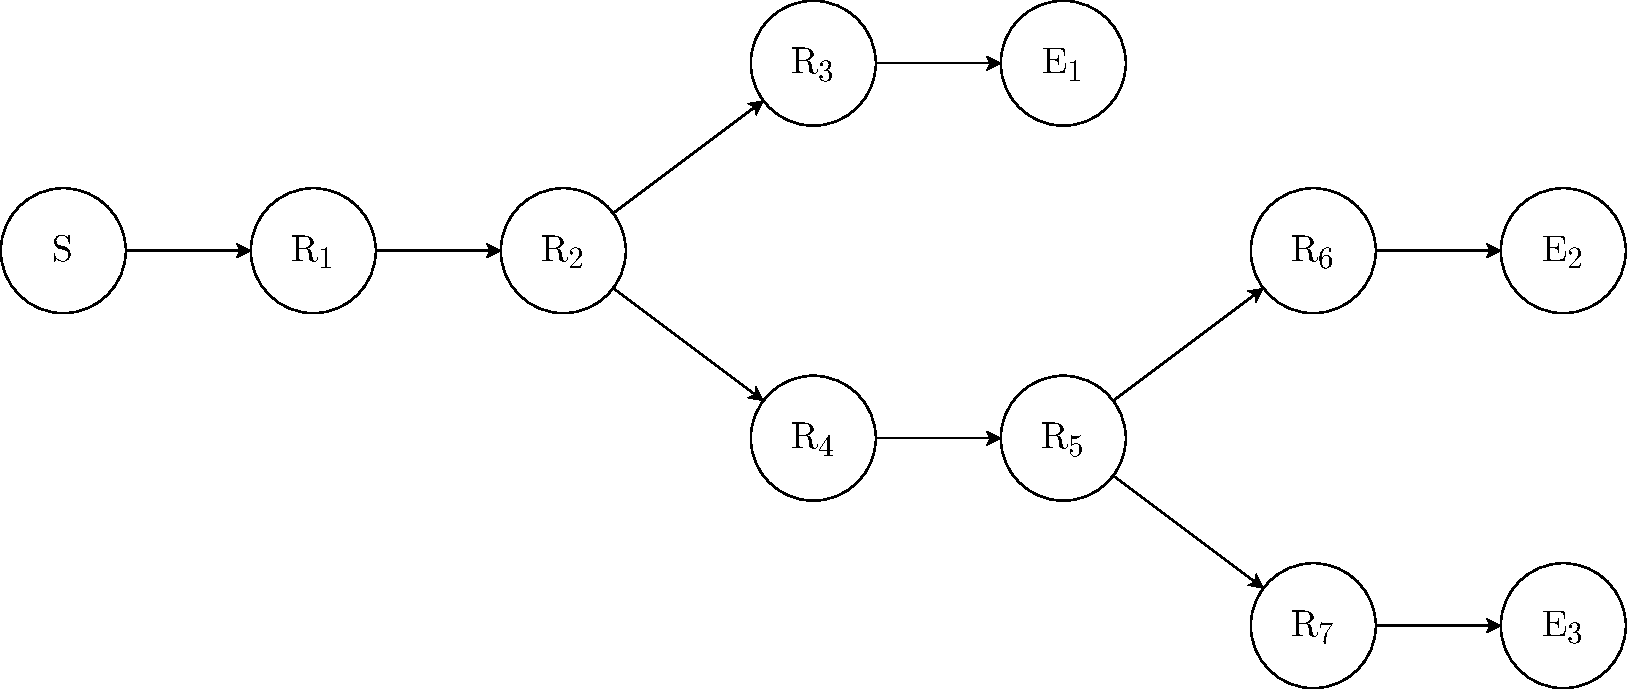
\includegraphics[width=.75\textwidth]{Bilder/xcast.pdf}
    \caption{Xcast processing (based on \cite{xcast_rfc})}
    \label{fig:xcast}
\end{figure}

For IPv6 \gls{xcast} is encoded in the routing extension header, optionally
    followed by a destination extension header specifying a port list,
    particularly in cases where receiver ports are diverging \cite{xcast_rfc}.
The IP destination field carries the \textit{``All-Xcast-Routers''} multicast
    address, necessitating  each \gls{xcast} router to join this multicast
    group.
As a result, each router is required to support \gls{xcast}.
For a gradual deployment, tunnel connections must be established between
    \gls{xcast} routers.
Alternatively, a tunnel connection can assembled to one \gls{xcast}-aware
    receiver.
This receiver has the capability to forward the packet either as an \gls{xcast}
    or IP unicast packet to the remaining endpoints \cite{xcast_rfc}.
% subsection Xcast (end)

\subsection{Explicit Multicast Extension} % (fold)
\label{sub:Explicit Multicast Extension}
There are several extensions to \gls{xcast}, one of which is known as
    \gls{xcast+} \cite{xcast+}.
A key enhancement of \gls{xcast+} is the reduction of the header overhead
    through the introduction of \glspl{dr} \cite{xcast+}.
The router nearest to a receiver determines itself as its \gls{dr}.
A client initiates the session by sending an IGMP ($S$, $G$) message ($S$:
    sender address, $G$: group address) to its \gls{dr}.
Upon receiving, the \gls{dr} sends a so-called \gls{xcast+} registration
    request message encompassing the sender's address ($S$), group address
    ($G$), and its own address towards the sender.
When the \gls{dr} at the sender's side receives it, it keeps track of all the
    \gls{dr} addresses interested in the multicast session ($S$, $G$).
When the sender transmits a multicast packet to its corresponding \gls{dr},
    it explicitly encodes the addresses of the \glspl{dr} at the receivers'
    side in the \gls{xcast} header and transmits the \gls{xcast+} packet, a
    process referred to as \gls{m2x}.
Consequently, \glspl{dr} are not stateless anymore.
Upon receiving \gls{xcast} packets, they perform a so-called \gls{x2m}
    transformation.
As a result, the corresponding address list of \gls{xcast+} might be
    significantly shorter compared to its \gls{xcast} alternative.

For instance in the scenario depicted in \autoref{fig:xcast}, $E_1$, $E_2$, and
    $E_3$ send an IGMP join message ($S$, $G$) to their respective \glspl{dr}
    $R_3$, $R_6$, and $R_7$.
Upon receiving, the receivers' side \glspl{dr} $R_3$, $R_6$, and $R_7$ send an
    \gls{xcast+} registration request ($S$, $G$, $R_i$) towards sender $S$.
When the \gls{dr} on the sender side receives the \gls{xcast+} registration
    requests, it adds a tuple for $R_3$, $R_6$, and $R_7$ encompassing ($S$,
    $G$, $R_i$) to its \gls{xcast+} table.
Upon receiving multicast packets from $S$, $R_1$ creates an \gls{xcast} packet
    with a destination list of \{$R_3$, $R_6$, $R_7$\}.
The processing of the intermediate nodes is identical to \gls{xcast}, expect 
    that no \gls{x2u} transmission is taken place.
When the client side \glspl{dr} $R_3$, $R_6$, and $R_7$ receive the packet, 
    they perform an \gls{x2m} transformation, sending a multicast packet to
    $E_1$, $E_2$, and $E_3$ respectively.
% subsection Explicit Multicast Extension (end)


\subsection{MEADcast} % (fold)
\label{sub:MEADcast}
% - Inspired by Xcast
% - designed to support a smooth transition from extensive unicast to
%   sender-centric multicast over the internet / across multiple
%   administrative domains
% - all information on the sender, routers are stateless
% - technology agnostic clients always receive IP Unicast
% - fallback mechanism
% - Given an initial list of receivers, the sender commences to send data in
%   unicast to each receiver while simultaneously probing the network for the
%   presence of MEADcast routers and hence for the option to consolidate
\gls{mead} is a sender-centric multicast protocol designed to facilitate a
    seamless transition from extensive unicast to multicast transmission
    \cite{meadcast2}.
The sender is responsible for all group management tasks, while the receivers
    consistently receive IP Unicast traffic, remaining agnostic to the use
    of MEADcast \cite{meadcast1}.
\gls{mead} endures across varying levels of network support, allowing for a
    gradual deployment of \gls{mead} router.
The protocol's design draws inspiration from \gls{xcast} \cite{meadcast1}.

\gls{mead} operates in two phases: discovery and data delivery.
On the sender side, this entails functionalities such as transmitting unicast
    and MEADcast packets as well as discovering \gls{mead} routers along the
    paths to receivers \cite{meadcast2}.
\gls{mead} routers, on the other hand, are responsible for forwarding and
    transforming \gls{mead} packets, as well as responding to and forwarding
    discovery requests \cite{meadcast2}.

\autoref{fig:mead_seq_dia} illustrates the interaction among the \gls{mead}
    sender, routers, and receivers: \cite{meadcast2}

\begin{enumerate}[label={(\arabic*)}]

\item
A session is established between the sender and the receivers.
\gls{mead} does not specify any mechanism for joining and leaving a session.
Therefore, an out-of-band session establishment is required, which can be based
    on a predefined receiver list on the sender or initiated by a request from
    a client.

\item
The sender initiates data transmission.
Due to the absence of a topology tree, data is transmitted via IP Unicast.
\gls{mead} routers forward IP Unicast packets as usual.

\item
Concurrently with step (2), the sender starts the initial discovery phase by
    transmitting discovery requests to all receivers.
Upon receiving discovery requests, a router sends a discovery response back to
    the sender and forwards the discovery request towards the designated
    receiver.
The router reads the hop count from the discovery request and increments it for
    both for the forwarded request and the discovery response.
If a client receives a discovery request, it ignores the packet.

\item
Upon receiving a discovery response, the sender inserts the router that sent
    the packet into its topology tree.
The topology tree is a graph with the sender as the root and the receivers as
    leaves.
\gls{mead} routers represent intermediate nodes, inserted at a position based
    on the hop count retrieved from the discovery response.

\item
After a predefined timeout is reached, the sender starts the data transmission
    phase by switching to \gls{mead} data delivery.
Until this point in time, the IP Unicast transmission continued in parallel
    with the discovery phase.
Receivers are grouped into \gls{mead} headers based on the current topology
    tree.
Each \gls{mead} router along a packet's path processes it based on the 
    information encoded in the \gls{mead} header.
It might forward the packet, create replicas, and forward them to other
    \gls{mead} routers, or perform a \gls{m2u} transformation, delivering the
    data to its destination.
\end{enumerate}

\begin{figure}
    \centering
    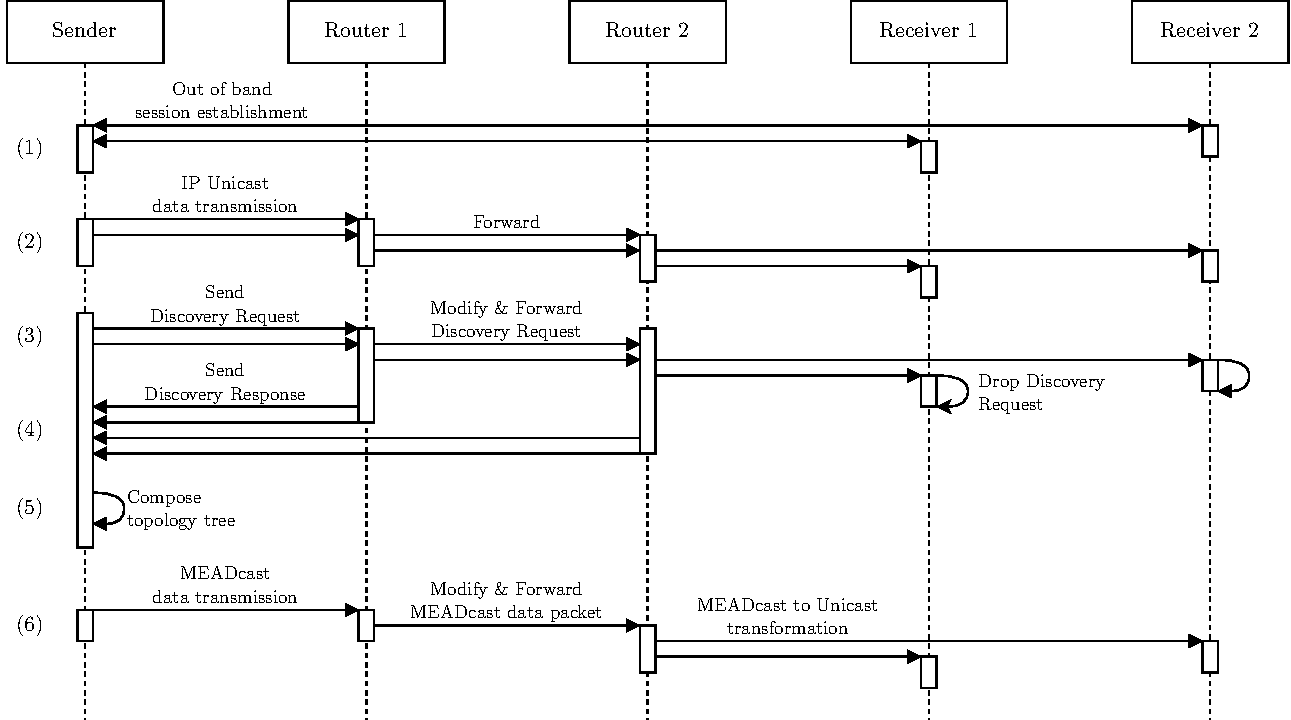
\includegraphics[width=.95\textwidth]{Bilder/mead_seq_dia.pdf}
    \caption{Interaction among participants in a MEADcast session (based on
        \cite{meadcast2})}
    \label{fig:mead_seq_dia}
\end{figure}

\paragraph{Protocol Header} % (fold)
\label{par:Protocol Header}
\gls{mead} is a multicast protocol based on IPv6 Unicast traffic.
In reference to \gls{xcast}, a list of receivers and their responsible
    \gls{mead} routers is encoded in the IPv6 routing header extension
    \cite{meadcast2}.
The Routing Header follows an IPv6 Hop-by-Hop extension header containing the
    Router Alert option\cite{meadcast2}.
Optionally, a port list encoded in the IPv6 Destination Option header may
    follows the Routing Header.
An optional port list encoded in the IPv6 destination option header may follows
    the Routing Header \cite{meadcast2}.
\autoref{fig:mead_hdr} attempts to illustrate the \gls{mead} header.
However, the papers about \gls{mead} \cite{meadcast1, meadcast2} lack an
    explicit specification of the header fields.
For instance, the content of the Router Alter Option Value, the Routing Type,
    and the Destination Option Header preamble are not specified.
Additionally, the size of the discovery flags and the \gls{mead} hops fields
    are not defined.
A brief description of each field is provided in
\autoref{tab:02_meadcast_header}.

\begin{figure}
\definecolor{lightgray}{gray}{0.8}
\begin{bytefield}[bitformatting=\tiny,bitwidth=1.1em,boxformatting=\centering\small]{32}
\bitheader{0-31} \\
\begin{rightwordgroup}{\small IPv6}
    % \bitbox{32}[bgcolor=lightgray]{} \\
    \bitbox{4}{Version} &
    \bitbox{8}{Traffic Class} &
    \bitbox{20}{Flow Label} \\
    \bitbox{16}{Payload Length} &
    \bitbox{8}{Next Header\\ \tiny (Hop-by-Hop: 0)} &
    \bitbox{8}{Hop Limit} \\
    \bitbox{32}{Source Address} \\
    \bitbox{32}{Destination Address}
\end{rightwordgroup} \\
\begin{rightwordgroup}{\small Hop-by-Hop}
    \bitbox{8}{Next Header\\ \tiny (Routing: 43)} &
    \bitbox{8}{Hdr Ext Len\\ \tiny (1)} &
    \bitbox{8}{Option Type\\ \tiny (Router Alert: 5)} &
    \bitbox{8}{Option Data Len\\ \tiny (2)} \\
    \bitbox{32}{Option Data}
    % \bitbox{16}[bgcolor=lightgray]{}
\end{rightwordgroup} \\
\begin{rightwordgroup}{\small MEADcast}
    \bitbox{8}{Next Header \\\tiny (e.g. Dst Opt: 60)} &
    \bitbox{8}{Hdr Ext Len} &
    \bitbox{8}{Routing Type} &
    \bitbox{8}{Num. Dst} \\
    \bitbox{2}{\tiny Dcvr Flags} &
    \bitbox{14}{Hops} &
    \bitbox{16}{Reserved} \\
    % \bitbox{16}[bgcolor=lightgray]{} \\
    \bitbox{32}{Delivery Bitmap} \\
    \bitbox{32}{Router Bitmap} \\
    \wordbox[lrt]{2}{Address List \\ \scriptsize (variable length)} \\
    \skippedwords\\
    \wordbox[lrb]{1}{}
    % \bitbox{32}{Destination Address 1} \\
    % \bitbox{32}{Destination Address 2} \\
    % \wordbox[]{1}{$\vdots$} \\[1ex]
    % \bitbox{32}{Destination Address N} \\
\end{rightwordgroup} \\
\begin{rightwordgroup}{Dst. Opt}
    \bitbox{8}{Next Header\\\tiny (e.g. UDP: 17)} &
    \bitbox{8}{Hdr Ext Len} &
    % \bitbox{16}[bgcolor=lightgray]{} \\
    \bitbox{8}{Option Type} &
    \bitbox{8}{Option Data Len} \\
    \bitbox{16}{Port 1} &
    \bitbox{16}{Port 2} \\
    \wordbox[]{1}{$\vdots$} \\[1ex]
    \bitbox{16}{Port N-1} &
    \bitbox{16}{Port N}
\end{rightwordgroup} \\
\end{bytefield}
    \caption[MEADcast Header]{MEADcast Header (based on \cite{meadcast2, meadcast1})}
    \label{fig:mead_hdr}
\end{figure}


\bgroup
\begin{table}[!htbp]
\centering
\def\arraystretch{1.35}%  1 is the default
\setlength{\tabcolsep}{1.2em}
\begin{tabularx}{\textwidth}{lX}
\toprule
\textbf{Field}& \textbf{Desciption} \\
\midrule
IPv6 src addr & A 32-bit field, carrying the senders IPv6 address
                \cite{meadcast2}.\\
IPv6 dst addr & A 32-bit field, carrying the IPv6 address of one receiver
                \cite{meadcast2}.\\ \midrule
Next Header   & An 8-bit selector, identifying the type of the immediately
                following header \cite{rfc8200_ipv6_hdr}.
                It employs identical values as the IPv4 Protocol field (e.g. 17
                = UDP, 59 = No Next Header for IPv6) \cite{iana_prot_nums}.
                The Hop-by-Hop header field carries 43, indicating the
                following routing header.
                The Routing Header field carries either 60 in cases of the
                presence of the optional port list, and otherwise, it carries 
                the number of the following Layer 3 protocol (e.g. 17 for
                \gls{udp}). \\
Hdr Ext Len   & An 8-bit unsigned integer representing the length of the
                Routing header in 8-octet units, excluding the initial 8
                octets \cite{rfc8200_ipv6_hdr}. \\
Routing Type  & An 8-bit identifier denoting a specific Routing header variant
                \cite{rfc8200_ipv6_hdr}.
                The \gls{mead} papers \cite{meadcast1,meadcast2} lack a
                specification of this field.\\
Num. Dst.     & Denotes the number of IPv6 addresses encoded in the address
                list.
                The size of this field lacks a specification.\\
Dcvr Flags    & Flags to mark a \gls{mead} packet as discovery request,
                response or data message \cite{meadcast2}.
                The size of the field lacks specification. \\
Hops          & Specifies the distance between the sender and a router, denoted
                in the number of MEADcast hops.
                This field is utilized during the discovery phase. The sender
                initializes the field with zero, and it is incremented by each
                intermediate MEADcast router encountered.
                The field size lacks specification.\\
Reserved      & A reserved field of unspecified size \cite{meadcast2}. \\
Delivery Map  & A 32-bit Bitmap, where each bit at position $i$ indicates
                whether a router at index $i$ in the address list has already
                been delivered (0 = delivered, 1 = not yet delivered)
                \cite{meadcast2}. \\
Router Map    & A 32-bit Bitmap, where each bit at position $i$ indicates
                whether an address at index $i$ in the address list is a
                router (0 = receiver, 1 = router) \cite{meadcast2}.\\
Address List  & A variable-length list comprising the IPv6 addresses of
                receivers and MEADcast routers \cite{meadcast2}. \\ \midrule
Dst Opt Preamble & The values for the Destination Option Preamble such as
                    Option Type and Option Data Len lack specification. \\
Port List     & A variable-length list encompassing the Layer 3 ports for each
                receiver in the address list \cite{meadcast2}.\\
\bottomrule
\end{tabularx}
\caption{MEADcast header field description}
\label{tab:02_meadcast_header}
\end{table}
\egroup
% paragraph Protocol Header (end)

\paragraph{Discovery Phase} % (fold)
\label{par:Discovery Phase}
The sender sends discovery requests of the form $req(E_i, d)$ ($E_i$ =
    receiver, d = distance) to all endpoints \cite{meadcast1}.
The routers respond to discovery requests with a disovery response
    $res(E_i, d, R_i)$ ($R_i$ = router).
Upon receiving a discovery response, the sender updates its topology tree in
    the following format: $(R_j,d_j,E_1^j,E_2^j)$.
For instance in the topology depicted in \autoref{fig:mead_delivery} the
    discovery phase look as follows:

\begin{enumerate}[label={(\arabic*)}]

\item
Sender $S$ start transmitting data to $E_1$, $E_2$, $E_3$, $E_4$, and $E_5$ via
    IP Unicast.

\item
$S$ sends a discovery request to each receiver, initialized with a distance of
    zero: $req(E_i, 0), i \in {1,2,3,4,5}$.

\item
Upon receiving the discovery requests, $R_1$ increments the hop counter and
    forwards the discovery requests: $req(E_i, 1), i \in {1,2,3,4,5}$.
    Additionally, for each discovery request $R_1$ sends a discovery response
        back to $S$: $res(E_i, 1, R_1), i \in {1,2,3,4,5}$.

\item
Step (3) is repeated on every router.

\item
Upon receiving discovery responses the clients ignore them.

\item
Upon receiving discovery responses $S$ updates its topology tree finally
        resulting in the following topology:
        ($R_1$, 1, $E_1$, $E_2$, $E_3$, $E_4$, $E_5$),
        ($R_2$, 2, $E_1$, $E_2$, $E_3$, $E_4$, $E_5$),
        ($R_3$, 3, $E_1$),
        ($R_4$, 3, $E_2$, $E_3$, $E_4$, $E_5$),
        ($R_5$, 4, $E_2$, $E_3$),
        ($R_6$, 4, $E_4$, $E_5$).

\item
After a predefined timeout is reached, the sender stops transmitting data and
    switches to the data transmission phase.
\end{enumerate}
% paragraph Discovery Phase (end)

\paragraph{Data Delivery} % (fold)
\label{par:Data Delivery}
During the data delivery phase, the receivers are grouped into \gls{mead}
    packets based on the topology tree constructed during the previous
    discovery phase \cite{meadcast1}.
The sender composes \gls{mead} data packet with an address list of the format
    $(R_j,E_1^j,E_2^j,\dots,R_k,E_1^k,E_2^k,\dots)$, with $R_j$ being the
    closest \gls{mead} router to $E_1^j$ and $E_2^j$ and $R_k$ being the
    closest router to $E_1^k$ and $E_2^j$.
The destination field of the IP header is set to the first receiver in the
    address list.

For the topology illustrated in \autoref{fig:mead_delivery}, sender $S$ the
    data delivery proceeds as follows:

\begin{enumerate}[label={(\arabic*)}]

\item
Sender $S$ transmits a \gls{mead} packet with an address list of
    $\{R_5,E_2,E_3,R_6,E_4,E_5\}$ and a destination IP address of $E_2$ to
    $R_1$.
The router bitmap is initialized to \texttt{"100100"}, indicating that the
    addresses at index 0 and 3 are \gls{mead} routers and addresses at index 1,
    2,4, and 5 are receivers.
Moreover, the bitmap specifies, that $R_5$ is responsible for $E_2$ and $E_3$,
    and $R_6$ is responsible or $E_4$ and $E_5$.
The delivery bitmap is initialized with the same value as the router bitmap,
    signaling no router has been delivered yet (1 = not delivered).
During delivery, the router bitmap is never altered.
Since $R_3$ is responsible only for one receiver, $E_1$ is served via IP
    Unicast, to save header space.

\item
Upon receiving the \gls{mead} data packet, $R_1$ parses the router and delivery
    bitmap.
For each undelivered router, specified by a set bit in both bitmaps, the router
    checks whether it is one of its own IP addresses.
If not, it creates a replica for each undelivered router.
For each replica, the bits of all other routers are set to zero in the delivery
    bitmap, and the destination IP is set to the first address following the
    router address.
In this scenario, $R_1$ parses the header and identifies an undelivered router
    address, which is $R_5$.
Since it is not its own address, $R_1$ creates a replica for $R_5$.
In the replica, the delivery bitmap is set to \texttt{"100000"}, and the
    destination IP is set to $E_2$.
Subsequently, $R_1$ identifies an undelivered router at index 3.
As it is the last router in the address list, no replica generation is
    necessary.
Instead the original packet can be modified, and the delivery bitmap is set to
    \texttt{"000100"}.
Finally, $R_1$ forwards the two \gls{mead} packets and the IP Unicast packet to
    $R_2$.
Since \gls{mead} endures partial network support and $R_1$ lacks knowledge of
    whether there is another \gls{mead} router along the path, which could
    instead perform the packet replication for $R_5$ and $R_6$.
For instance, $R_2$, $R_3$, and $R_4$ could be non-\gls{mead} routers.
Consequently, $R_1$ sends separate replicas for $R_5$ and $R_6$, despite their
    shared path of \gls{mead} routers until $R_4$.

\item
Upon receiving the \gls{mead} packets, $R_2$ parses the header of both packets.
Since the only router address in each packet is not owned by $R_2$, it just
    forwards both packets.
The IP Unicast packet to $E_1$ is forwarded as usual.
When $R_3$ receives the unicast packet, it delivers it to $E_1$.

\item
Upon receiving the \gls{mead} packets, $R_4$ parses the header of both packets.
Since the only router address in each packet is not owned by $R_4$, it just
    forwards both packets to $R_5$ and $R_6$ respectively.

\item
Upon receiving the \gls{mead} packet, $R_5$ and $R_6$ parse the header,
    identifying their own address as the only undelivered router in the address
    list.
Consequently, both routers perform an \gls{m2u} transformation for each address
    following their own address.
This involves creating an IP packet for each receiver, with the destination
    address set to the receiver's address.
If the \gls{mead} packet includes the optional port list, the port in the Layer
    3 header is set to the respective port from the list.
If the Layer 3 protocol encompasses a checksum, it must be corrected, due to
    the alteration of the IP pseudo-header.
For $R_5$, this process continues until another router address is encountered
at index 3, while for $R_6$, it continues until the last index of the list.
Subsequently, they each send IP Unicast packets to their respective
    destinations: $E_2$ and $E_3$ for $R_5$, and $E_4$ and $E_5$ for $R_6$.
\end{enumerate}

% paragraph Data Delivery (end)

\begin{figure}
\centering
\begin{forest}
    for tree={grow=east, circle, draw, font=\footnotesize, l sep=14ex},
        where level=0{minimum size=2em}{},
        where level=2{
            s sep+=36pt
        }{},
        where level=4{l sep-=40}{},
        where={n_children==0}{font=\scriptsize, edge=dashed}{}
    [$S$
        [$R_1$,
            edge label={node[midway,above=3mm,font=\tiny,align=center]{
                Unicast: \{$E_1$\}\\
                \{$\underline{R_5}$,$E_2$,$E_3$,$\underline{R_6}$,$E_4$,$E_5$\}
            }}
            [$R_2$,
            edge label={node[midway,above=3mm,font=\tiny,align=center]{
                Unicast: \{$E_1$\}\\
                \{$\underline{R_5}$,$E_2$,$E_3$,$\underline{\cancel{R_6}}$,
                    $\cancel{E_4}$,$\cancel{E_5}$\}\\
                \{$\underline{\cancel{R_5}}$,$\cancel{E_2}$,$\cancel{E_3}$,
                    $\underline{R_6}$,$E_4$,$E_5$\}
            }}
                [$R_4$,
            edge label={node[midway,above,sloped,font=\tiny,align=left]{
                \{$\underline{R_5}$,$E_2$,$E_3$,$\underline{\cancel{R_6}}$,
                    $\cancel{E_4}$,$\cancel{E_5}$\}\\
                \{$\underline{\cancel{R_5}}$,$\cancel{E_2}$,$\cancel{E_3}$,
                    $\underline{R_6}$,$E_4$,$E_5$\}
            }}
                    [$R_6$,
                        edge label={node[midway,below=2mm,sloped,font=\tiny,align=center]{
                            \{$\underline{\cancel{R_5}}$,$\cancel{E_2}$,$\cancel{E_3}$,
                                $\underline{R_6}$,$E_4$,$E_5$\}
                        }}
                        [$E_5$,
                            edge label={node[midway,above=1mm,align=center,font=\tiny]{unicast}}
                        ][$E_4$]
                    ]
                    [$R_5$,
                        edge label={node[midway,above,sloped,font=\tiny,align=center]{
                            \{$\underline{R_5}$,$E_2$,$E_3$,$\underline{\cancel{R_6}}$,
                                $\cancel{E_4}$,$\cancel{E_5}$\}\\
                        }}
                        [$E_3$,
                            edge label={node[midway,above=1mm,align=center,font=\tiny]{unicast}}
                        ][$E_2$]
                    ]
                ]
                [$R_3$,
                    edge label={node[midway,above,sloped,font=\tiny,align=center]{
                        Unicast: \{$E_1$\}
                    }}
                    [$E_1$,
                        edge label={node[midway,above,align=center,font=\tiny]{unicast}}
                    ]
                ]
            ]
        ]
    ]
\end{forest}
\caption[MEADcast data delivery]{
    MEADcast Data Delivery:
    An underscored address signifies a set bit in the router bitmap, while a
        stroked-through address indicates that the corresponding router bit is
        set to ``delivered'' (0) in the delivery bitmap.
    }
\label{fig:mead_delivery}
\end{figure}

% subsection MEADcast (end)
% section Mutlicast (end)

\section{Hierachical Three-Layer Internetworking Model} % (fold)
\label{sec:Hierachical Three-Layer Internet Model}
% First, this section introduces state-of-the-art characteristics of medium to
%     large-sized network architectures.
% Subsequently, we delve into the network topology of our testbed.
Since, we this thesis we design a medium-sized network topology, this section 
    introduces state-of-the-art characteristics of medium to large-sized
    network architectures.

Several fundamental design principles must be met by any network, irrespective
    of its size \cite{cisco_net_size}.
These principles are mutually interdependent and also tightly coupled to the
    overall design \cite{cisco_campus_net}.

% \textit{Hierarchy}:
\paragraph{Hierarchy} % (fold)
\label{par:Hierarchy}
A hierarchical network model serves as a crucial high-level
    tool for crafting a reliable network topology \cite{cisco_net_size}.
This abstraction dissects the complex challenge of network design into smaller
    and more manageable areas.
A significant advantage of a hierarchical topology is that local traffic
    is confined to the local network \cite{cisco_campus_net}.
Only traffic destined for other networks is transferred to a higher layer.

% paragraph Hierarchy (end)

% \textit{Modularity}:
\paragraph{Modularity} % (fold)
\label{par:Modularity}
Dividing the network into components provides numerous benefits.
First, each component or module can be designed with a level of independence
    from the overall structure \cite{cisco_net_size}.
All modules can operate as semi-independent elements, contributing to higher
    overall system availability and facilitating simpler management and
    operations \cite{cisco_campus_net}.
Furthermore, network changes and upgrades can be applied in a controlled and
    staged manner, enhancing flexibility in maintaining and operating the
    network \cite{cisco_net_size}.
This principle has also been leveraged in software architecture for many years,
    by separating the application into presentation, logic, and data layers
    \cite{sw_arch}.
Another benefit is a higher degree of isolation, confining problems and
    failures to their component, leaving the overall network unaffected
    \cite{cisco_design_guide}.
In summary, dividing a network into a set of assembled building blocks
    facilitates increased stability, flexibility, and manageability for both
    the individual components and the network as a whole.
    \cite{cisco_campus_net}
% paragraph Modularity (end)

% \textit{Resiliency}:
\paragraph{Resiliency} % (fold)
\label{par:Resiliency}
The network is expected to sustain availability for both
    regular and irregular scenarios.
Typical scenarios encompass anticipated traffic flows, expected traffic
    patterns, and scheduled events like maintenance windows
    \cite{cisco_net_size}.
Abnormal scenarios involve hardware or software failures, high traffic loads,
    anomalous traffic patterns, \gls{dos} events, and other unforeseen
    circumstances \cite{cisco_campus_net}.
% paragraph Resiliency (end)

% \textit{Flexibility}:
\paragraph{Flexibility} % (fold)
\label{par:Flexibility}
As the operational lifespan of networks extends, it becomes imperative for
    their design to facilitate enhanced adaptability and flexibility
    \cite{cisco_campus_net}.
Adapting to evolving business environments and their associated communication
    requirements is a practical business and operational necessity.
Flexibility is the capacity to modify specific sections of the network,
    introduce new services, or enhance capacity without necessitating a
    substantial overhaul or replacement of major hardware devices
    \cite{cisco_net_size}.
% paragraph Flexibility (end)

To meet these ubiquitous network requirements, \citeauthor{cisco_3_tier}
    \cite{cisco_3_tier} first proposed the \textit{hierarchical three-layer
    internetworking model} in \citeyear{cisco_3_tier}.
This model has evolved into an industry-wide standard for designing reliable,
    scalable, and cost-efficient networks \cite{cisco_net_size}.
Leading networking and telecommunication providers like Cisco and Huawei
    recommend the implementation of the hierarchical three-layer
    internetworking model.
    \cite{cisco_campus_net,huawei_campus_net}.
The model divides networks into three layers: core, distribution, and access
    as illustrated in \autoref{fig:three-layer} \cite{cisco_3_tier}.

% \textit{Access Layer}:
\paragraph{Access Layer} % (fold)
\label{par:Access Layer}
The access layer facilitates network access for end devices, encompassing PCs,
    smartphones, printers, and IP cameras \cite{cisco_net_size}.
Operating commonly at layer 2, it establishes connectivity between end devices.
Given the diverse range of end devices, this layer incorporates an array of
    network devices such as switches, access points, and routers
    \cite{cisco_campus_net}.
Serving as the demarcation point between the network infrastructure and
    computing devices \cite{cisco_campus_net}, the access layer acts as the
    initial security boundary, safeguarding other users, application resources,
    and the network itself \cite{cisco_design_guide}.
% paragraph Access Layer (end)

% \textit{Distribution Layer}:
\paragraph{Distribution Layer} % (fold)
\label{par:Distribution Layer}
The distribution layer aggregates traffic from multiple access layer devices
    and provides connectivity to the rest of the network by transmitting
    packets to other access layer devices or the core layer
    \cite{cisco_campus_net}.
In a typical scenario, connected routers at the distribution layer aggregate
    data originating from a building or a floor and establish connections to
    the core layer.
For instance, in \autoref{fig:three-layer}, the two interconnected routers on
    the left and the two on the right could each symbolize a distinct building.
This layer often serves as the demarcation between layer 2 domains and the
    layer 3 routed network \cite{cisco_net_size}, creating fault domains
    containing failures and network changes to the directly affected areas
    \cite{cisco_design_guide}.
The distribution layer performs essential network functions such as routing,
    traffic filtering, and policy enforcement \cite{cisco_campus_net}.
% paragraph Distribution Layer (end)


% \textit{Core Layer}:
\paragraph{Core Layer} % (fold)
\label{par:Core Layer}
Core LayerThe core layer functions as the backbone interconnecting the numerous modules
    of the network \cite{cisco_campus_net}.
It facilitates connectivity among end devices, servers, data storage, different
    locations, and the internet.
This layer represents the most critical component of the network, characterized
    by a relatively simple design \cite{cisco_design_guide}.
Given that a significant portion of network traffic passes through the
    backbone, it is responsible for high-speed and high-volume data
    transmission \cite{cisco_campus_net}.
Additionally, this layer should offer high availability and redundancy.
CPU-intensive packet manipulations resulting from security measures,
    inspections, and \gls{qos} should be avoided \cite{cisco_campus_net}.
% paragraph Core Later (end)


\begin{figure}
    \begin{center}
        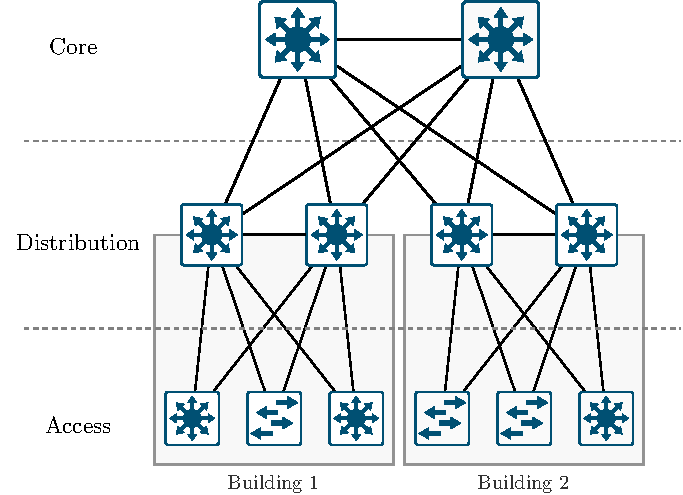
\includegraphics[width=.6\textwidth]{three_layer_model.pdf}
    \end{center}
    \caption{Hierarchical three-layer internetworking model (based on
    \cite{cisco_3_tier})}
    \label{fig:three-layer}
\end{figure}

% section Hierachical Three-Layer Internetworking Model (end)

% chapter Background Work (end)
